\documentclass[portuguese]{sbc2025}%

\usepackage[misc,geometry]{ifsym}

\raggedbottom  % Prevent underfull vbox warnings

\usepackage{aas_macros}
\usepackage[bottom]{footmisc}

\usepackage{tabularray}
\usepackage{adjustbox}
\usepackage{stfloats}

\usepackage{afterpage}
\usepackage{url}
\usepackage{pifont}

\setcitestyle{square}

\definecolor{engtitle}{rgb}{0.5,0.5,0.5}
\definecolor{orcidlogo}{rgb}{0.37,0.48,0.13}
\definecolor{unilogo}{rgb}{0.16, 0.26, 0.58}
\definecolor{maillogo}{rgb}{0.58, 0.16, 0.26}
\definecolor{darkblue}{rgb}{0.0,0.0,0.0}
\hypersetup{colorlinks,breaklinks,
            linkcolor=darkblue,urlcolor=darkblue,
            anchorcolor=darkblue,citecolor=darkblue}

\jyear{2025}

\category{Artigo de Pesquisa/Research Paper}
\title[Sistema de Monitoria-IC: Plataforma Web para Gestão de Monitorias Acadêmicas da UFBA]{Sistema de Monitoria-IC: Plataforma Web para Gestão Completa de Monitorias Acadêmicas da UFBA}
\engtitle{\textcolor{engtitle}{Sistema de Monitoria-IC: Web Platform for Complete Management of Academic Monitoring Programs at UFBA}}

\author[Sena et al. 2025]{
\affil{\textbf{Luis Felipe Cordeiro Sena}~\orcidlink{0009-0009-3997-3639}~\textcolor{blue}{\faEnvelopeO}~~[{Universidade Federal da Bahia}~|\href{mailto:luis.sena@ufba.br}{~{\textit{luis.sena@ufba.br}}}~]}

\affil{\textbf{Frederico Araújo Durão}~\orcidlink{0000-0002-7766-6666}~~[{Universidade Federal da Bahia}~| \href{mailto:fdurao@ufba.br}{{\textit{fdurao@ufba.br}}}~]}
}

\begin{document}

\begin{frontmatter}

\maketitle

\begin{mail}
Instituto de Computação, Universidade Federal da Bahia, Av. Milton Santos, s/n - Campus de Ondina, PAF 2, Salvador, BA, 40170-110, Brasil.
\end{mail}

\begin{abstract-pt}
A monitoria acadêmica é um processo fundamental nas universidades brasileiras que permite aos alunos desenvolverem habilidades pedagógicas enquanto auxiliam no processo de ensino-aprendizagem. Porém, o gerenciamento desse processo frequentemente enfrenta desafios relacionados à burocracia, falta de transparência e múltiplos processos manuais ineficientes. Este trabalho apresenta o desenvolvimento do Sistema de Monitoria-IC, uma plataforma web projetada para automatizar e simplificar todo o ciclo de vida dos projetos de monitoria na UFBA. A solução proposta digitaliza desde a criação de projetos pelos professores até a seleção de monitores, alocação de bolsas e geração de relatórios finais. O sistema foi desenvolvido utilizando tecnologias modernas como Next.js 15, TypeScript, tRPC, PostgreSQL e MinIO, seguindo princípios de engenharia de software que garantem escalabilidade e manutenibilidade. A arquitetura implementada separa claramente as responsabilidades entre um Sistema de Processamento de Transações (SPT) para operações cotidianas e funcionalidades gerenciais para análise e controle. A validação técnica através de testes end-to-end demonstra a robustez da solução. Os resultados indicam que a automação proposta elimina retrabalho administrativo, aumenta a transparência através de histórico auditável, e estabelece uma base sólida para modernização da gestão acadêmica na universidade. O sistema encontra-se disponível em produção em https://sistema-de-monitoria.app.ic.ufba.br/.
\end{abstract-pt}

\begin{abstract-en}
Academic monitoring is a fundamental process in Brazilian universities that allows students to develop pedagogical skills while assisting in the teaching-learning process. However, managing this process often faces challenges related to bureaucracy, lack of transparency, and multiple inefficient manual procedures. This work presents the development of Sistema de Monitoria-IC, a web platform designed to automate and simplify the entire lifecycle of monitoring projects at UFBA. The proposed solution digitizes everything from project creation by professors to monitor selection, scholarship allocation, and final report generation. The system was developed using modern technologies such as Next.js 15, TypeScript, tRPC, PostgreSQL, and MinIO, following software engineering principles that ensure scalability and maintainability. The implemented architecture clearly separates responsibilities between a Transaction Processing System (TPS) for daily operations and managerial functionalities for analysis and control. Technical validation through end-to-end tests demonstrates the solution's robustness. Results indicate that the proposed automation eliminates administrative rework, increases transparency through auditable history, and establishes a solid foundation for modernizing academic management at the university. The system is available in production at https://sistema-de-monitoria.app.ic.ufba.br/.
\end{abstract-en}

\begin{pchaves}
Gestão Acadêmica, Sistema de Monitoria, Arquitetura de Software, Desenvolvimento Web, Automação de Processos.
\end{pchaves}

\begin{keywords}
Academic Management, Monitoring System, Software Architecture, Web Development, Process Automation.
\end{keywords}

\begin{dates}
% Informações serão preenchidas pelo editor antes da publicação
\end{dates}

\end{frontmatter}

\section{Introdução}
\label{sec:intro}

\subsection{Contextualização e Motivação}

A monitoria acadêmica representa um dos pilares fundamentais do ensino superior brasileiro, estabelecendo-se como uma prática pedagógica que beneficia simultaneamente monitores, estudantes e docentes. Regulamentada pela Lei nº 9.394/96 (Lei de Diretrizes e Bases da Educação Nacional), a monitoria permite que alunos com destacado desempenho acadêmico auxiliem seus pares no processo de aprendizagem, desenvolvendo competências didáticas enquanto aprofundam seus conhecimentos na disciplina \cite{Brasil1996}.

Na Universidade Federal da Bahia (UFBA), o programa de monitoria segue um fluxo complexo que envolve múltiplos atores e etapas interdependentes. O processo inicia-se com o planejamento semestral, quando a administração importa dados de disciplinas e professores. Em seguida, os docentes criam e submetem projetos de monitoria que precisam ser aprovados administrativamente. Após a aprovação, ocorre a publicação de editais internos, inscrição de candidatos, processo seletivo, alocação de bolsas, e finalmente, a consolidação de dados para envio à PROGRAD (Pró-Reitoria de Graduação).

Apesar de sua importância reconhecida, a gestão dos programas de monitoria na UFBA ainda depende predominantemente de processos manuais e fragmentados. Formulários em papel, planilhas eletrônicas dispersas, comunicação via e-mail e ausência de um sistema centralizado caracterizam o cenário atual, resultando em ineficiências operacionais significativas. Essa realidade contrasta com a tendência global de digitalização e automação de processos administrativos no ambiente acadêmico, conforme defendem \cite{Laudon_Laudon_2011}, que argumentam que a tecnologia da informação constitui uma das principais ferramentas para alcançar excelência operacional.

\subsection{Identificação do Problema}

O processo tradicional de gestão de monitoria apresenta diversos problemas críticos que impactam negativamente todos os envolvidos no programa:

\textbf{Para os Professores:}
\begin{itemize}
  \item Tempo excessivo gasto com tarefas burocráticas repetitivas
  \item Dificuldade em reutilizar templates de projetos de semestres anteriores
  \item Processo de seleção manual e demorado, com análise individual de documentos
  \item Falta de ferramentas adequadas para acompanhamento das atividades dos monitores
  \item Necessidade de gerar relatórios finais manualmente ao término do semestre
\end{itemize}

\textbf{Para os Estudantes:}
\begin{itemize}
  \item Descoberta de oportunidades através de canais fragmentados (murais, e-mails esporádicos)
  \item Processo de inscrição com múltiplos formulários e envio de documentos por diferentes meios
  \item Falta de transparência no processo seletivo e incerteza quanto ao status da candidatura
  \item Dificuldade em acompanhar resultados e prazos importantes
  \item Ausência de histórico centralizado de participações anteriores
\end{itemize}

\textbf{Para a Administração:}
\begin{itemize}
  \item Retrabalho constante na consolidação de dados de diferentes fontes
  \item Dificuldade em garantir conformidade com prazos e regulamentos
  \item Ausência de dados consolidados para planejamento estratégico
  \item Compilação manual de relatórios para órgãos superiores
  \item Impossibilidade de análises históricas e métricas de desempenho do programa
\end{itemize}

\subsection{Objetivos}

Este trabalho documenta o desenvolvimento e implementação do \textbf{Sistema de Monitoria-IC}, uma plataforma web completa para gestão dos projetos de monitoria do Instituto de Computação da UFBA. O objetivo central é substituir fluxos manuais e dispersos por um sistema único que garanta transparência, rastreabilidade e padronização de todo o processo de monitoria.

Os objetivos específicos incluem:

\begin{enumerate}
  \item \textbf{Digitalizar o ciclo completo de projetos de monitoria:} desde a criação com templates reutilizáveis, assinatura digital pelo professor, submissão, até aprovação administrativa e publicação de editais

  \item \textbf{Automatizar o processo seletivo:} permitindo inscrições online, captura automática de notas e CR do histórico, consideração de equivalências entre disciplinas, e publicação transparente de resultados

  \item \textbf{Sistematizar a alocação de bolsas:} com geração automática de planilhas para o Instituto, configuração do total de bolsas informado pela PROGRAD, e alocação por projeto com validações automáticas

  \item \textbf{Eliminar trabalhos manuais repetitivos:} através de automação de notificações por e-mail, geração de documentos PDF, e integração com armazenamento de arquivos

  \item \textbf{Fornecer base analítica para tomada de decisões:} com dashboards administrativos, APIs para integração, e relatórios consolidados para análises institucionais
\end{enumerate}

\subsection{Estrutura do Artigo}

Este artigo está organizado da seguinte forma: a Seção 2 apresenta os fundamentos teóricos sobre Sistemas de Informação e monitoria acadêmica. A Seção 3 analisa trabalhos relacionados e o estado da prática em universidades brasileiras. A Seção 4 detalha a arquitetura, tecnologias e implementação do Sistema de Monitoria-IC. A Seção 5 apresenta os resultados obtidos e discussões. Por fim, a Seção 6 conclui o trabalho e aponta direções futuras.

\section{Fundamentação Teórica}
\label{sec:background}

\subsection{Monitoria Acadêmica no Ensino Superior Brasileiro}

A monitoria acadêmica constitui uma modalidade de ensino-aprendizagem que contribui para a formação integrada do aluno nas atividades de ensino, pesquisa e extensão dos cursos de graduação. Conforme estabelecido pela Lei de Diretrizes e Bases da Educação Nacional (Lei nº 9.394/96), as universidades devem aproveitar estudantes de bom rendimento acadêmico em tarefas de ensino e pesquisa \cite{Brasil1996}.

O processo de monitoria na UFBA segue diretrizes institucionais específicas que definem:
\begin{itemize}
  \item Critérios de seleção baseados em desempenho acadêmico (nota na disciplina e Coeficiente de Rendimento)
  \item Modalidades de participação (bolsista ou voluntário)
  \item Responsabilidades do monitor, professor orientador e coordenação
  \item Fluxo de aprovação de projetos e alocação de recursos
  \item Requisitos para certificação ao final do período
\end{itemize}

Estudos sobre programas de monitoria demonstram benefícios significativos: desenvolvimento de habilidades didáticas nos monitores \cite{Natario2010}, melhoria no desempenho acadêmico dos estudantes assistidos \cite{Frison2016}, e apoio essencial aos docentes na condução de atividades práticas \cite{Dantas2014}. Entretanto, esses mesmos estudos apontam desafios na gestão administrativa desses programas, especialmente relacionados à burocracia e falta de ferramentas adequadas.

\subsection{Sistemas de Informação na Gestão Acadêmica}

\subsubsection{Sistemas de Processamento de Transações (SPT)}

Conforme \cite{Laudon_Laudon_2011}, os SPTs são "sistemas informatizados que realizam e registram as transações rotineiras necessárias ao funcionamento organizacional". No contexto acadêmico, esses sistemas gerenciam operações como matrículas, lançamento de notas, controle de frequência e, no caso específico deste trabalho, o ciclo de vida dos projetos de monitoria.

As características essenciais de um SPT incluem:
\begin{itemize}
  \item Alta precisão e confiabilidade nos dados
  \item Processamento rápido de grande volume de transações
  \item Capacidade de auditoria e rastreabilidade
  \item Disponibilidade contínua para operações críticas
\end{itemize}

\subsubsection{Sistemas de Informações Gerenciais (SIG)}

Os SIGs, segundo \cite{Laudon_Laudon_2011}, "resumem e relatam as operações básicas da empresa usando dados fornecidos pelos SPTs". No Sistema de Monitoria-IC, o componente SIG oferece dashboards, relatórios consolidados e métricas que permitem à administração:
\begin{itemize}
  \item Monitorar o andamento dos processos de monitoria
  \item Analisar tendências históricas de participação
  \item Avaliar a distribuição de recursos entre departamentos
  \item Gerar relatórios para órgãos superiores
\end{itemize}

\subsubsection{Arquitetura Híbrida SPT-SIG}

A separação de responsabilidades entre SPT (camada operacional) e SIG (camada analítica) fundamenta a arquitetura do Sistema de Monitoria-IC. O SPT gerencia o ciclo de vida de cada transação – cadastros, aprovações, inscrições – enquanto o SIG consome os registros consolidados para gerar análises e relatórios. Essa divisão promove:
\begin{itemize}
  \item Escalabilidade independente de cada camada
  \item Facilidade de manutenção e evolução
  \item Redução do acoplamento entre operações e análises
  \item Melhor desempenho através de otimizações específicas
\end{itemize}

\subsection{Tecnologias Modernas para Desenvolvimento Web}

O desenvolvimento de aplicações web modernas beneficia-se de frameworks e ferramentas que promovem produtividade, manutenibilidade e desempenho. As principais tecnologias utilizadas neste projeto incluem:

\textbf{Next.js e React:} Framework full-stack que combina renderização no servidor (SSR) e no cliente (CSR), otimizando desempenho e SEO enquanto mantém a reatividade característica de Single Page Applications \cite{Vercel2024}.

\textbf{TypeScript:} Superset tipado de JavaScript que adiciona verificação estática de tipos, reduzindo erros em tempo de execução e melhorando a manutenibilidade do código \cite{Microsoft2024}.

\textbf{tRPC:} Biblioteca que permite criar APIs type-safe sem necessidade de geração de código ou schemas compartilhados, garantindo consistência entre cliente e servidor \cite{TRPC2024}.

\textbf{PostgreSQL e Drizzle ORM:} Banco de dados relacional robusto combinado com um ORM TypeScript-first que oferece type safety e migrações automáticas \cite{PostgreSQL2024, Drizzle2024}.

\section{Trabalhos Relacionados}
\label{sec:related-work}

\subsection{Sistemas de Gestão Acadêmica Generalistas}

Diversos sistemas de gestão acadêmica são utilizados em universidades brasileiras, como o SIGAA (Sistema Integrado de Gestão de Atividades Acadêmicas) desenvolvido pela UFRN e adotado por várias instituições federais \cite{UFRN2024}. Embora esses sistemas ofereçam módulos abrangentes para gestão universitária, frequentemente carecem de funcionalidades específicas para o workflow detalhado de programas de monitoria.

O SIGA (Sistema Integrado de Gestão Acadêmica) da UFRJ e o Sistema Acadêmico da USP (Júpiter) são outros exemplos de soluções institucionais que, apesar de robustas, não cobrem adequadamente aspectos como:
\begin{itemize}
  \item Templates reutilizáveis de projetos de monitoria
  \item Assinatura digital com diferentes papéis (professor, chefe de departamento)
  \item Processo seletivo com critérios customizáveis por projeto
  \item Consideração automática de equivalências entre disciplinas
  \item Geração de consolidações específicas para PROGRAD
\end{itemize}

\subsection{Levantamento do Estado da Prática}

Para avaliar o estado atual da gestão de monitoria em universidades brasileiras, realizamos um levantamento nos cursos de Computação das dez universidades públicas mais bem classificadas segundo o Ranking Universitário Folha (RUF) 2024 \cite{folha2024ruf}.

\begin{table*}[htb]
  \centering
  \caption{Panorama da gestão de monitoria em universidades públicas brasileiras}
  \label{tab:estado-pratica}
  \begin{adjustbox}{max width=\textwidth}
    \begin{tabular}{|c|l|c|c|p{3cm}|p{5cm}|}
      \hline
      \textbf{Rank} & \textbf{Universidade} & \textbf{Sistema Específico} & \textbf{Sistema Integrado} & \textbf{Ferramentas} & \textbf{Características} \\
      \hline
      1º & USP & Não & Parcial & Júpiter + Forms & Cadastro no sistema acadêmico, seleção via formulários \\
      \hline
      2º & Unicamp & Não & Não & E-mail + Planilhas & Processo totalmente manual \\
      \hline
      3º & UFRGS & Não & Sim & Portal do Aluno & Funcionalidades básicas no portal institucional \\
      \hline
      4º & UFRJ & Não & Parcial & SIGA + E-mail & Registro no SIGA, processo seletivo manual \\
      \hline
      5º & UFMG & Não & Não & Google Forms & Inscrições via formulários, gestão em planilhas \\
      \hline
      6º & UNESP & Não & Não & E-mail + Docs & Processo manual com documentos Word \\
      \hline
      7º & UFSC & Não & Sim & CAGR & Sistema acadêmico com módulo básico \\
      \hline
      8º & UnB & Não & Parcial & SIGAA & Módulo genérico no SIGAA \\
      \hline
      9º & UNIFESP & Não & Não & SEI + Forms & Processo administrativo via SEI \\
      \hline
      10º & UFPR & Não & Não & Microsoft Forms & Formulários online, gestão manual \\
      \hline
    \end{tabular}
  \end{adjustbox}
\end{table*}

Os resultados revelam que:
\begin{itemize}
  \item \textbf{Nenhuma instituição} possui sistema específico e completo para gestão de monitoria
  \item 70\% utilizam ferramentas genéricas (Google/Microsoft Forms, e-mail)
  \item Apenas 30\% possuem alguma integração com sistemas acadêmicos existentes
  \item Todos os processos seletivos envolvem etapas manuais significativas
  \item Não há padronização ou compartilhamento de soluções entre instituições
\end{itemize}

\subsection{Análise Comparativa}

A análise dos trabalhos relacionados e do estado da prática revela uma lacuna significativa: enquanto existem sistemas acadêmicos robustos para gestão geral, falta uma solução específica que atenda às particularidades do processo de monitoria. O Sistema de Monitoria-IC diferencia-se por:

\begin{enumerate}
  \item \textbf{Especificidade:} Desenvolvido especificamente para o workflow de monitoria, não como módulo genérico
  \item \textbf{Completude:} Cobre todo o ciclo de vida, da criação de projetos à emissão de certificados
  \item \textbf{Automação:} Elimina etapas manuais através de integrações e processamento inteligente
  \item \textbf{Modernidade:} Utiliza stack tecnológico atual com foco em UX e performance
  \item \textbf{Transparência:} Oferece rastreabilidade completa e acesso diferenciado por papéis
\end{enumerate}

\section{Sistema de Monitoria-IC}
\label{sec:system}

\subsection{Visão Geral da Arquitetura}

O Sistema de Monitoria-IC foi projetado seguindo uma arquitetura em camadas que separa claramente as responsabilidades e promove manutenibilidade e escalabilidade. A arquitetura segue o padrão de três camadas com componentes especializados:

\subsubsection{Camada de Apresentação}

Implementada como uma Single Page Application (SPA) usando Next.js 15, React e TypeScript. Principais características:
\begin{itemize}
  \item Interface responsiva com componentes shadcn/ui e Tailwind CSS
  \item Roteamento dinâmico com proteção baseada em papéis
  \item Gerenciamento de estado com React Query e Zustand
  \item Validação de formulários com React Hook Form e Zod
\end{itemize}

\subsubsection{Camada de Aplicação}

Utiliza tRPC v11 para criar uma API type-safe entre cliente e servidor:
\begin{itemize}
  \item Procedures organizados por domínio (projeto, inscricao, edital, etc.)
  \item Middleware de autenticação com Lucia Auth
  \item Validação automática de entrada/saída com Zod
  \item Suporte a subscriptions para atualizações em tempo real
\end{itemize}

\subsubsection{Camada de Negócio}

Implementa a lógica central do sistema através de serviços especializados:
\begin{itemize}
  \item \texttt{ProjectService}: Gerencia ciclo de vida dos projetos
  \item \texttt{SelectionService}: Processa inscrições e seleções
  \item \texttt{NotificationService}: Envia e-mails automatizados
  \item \texttt{DocumentService}: Gera PDFs e gerencia assinaturas
  \item \texttt{AnalyticsService}: Consolida dados para relatórios
\end{itemize}

\subsubsection{Camada de Dados}

PostgreSQL com Drizzle ORM para persistência e MinIO para armazenamento de objetos:
\begin{itemize}
  \item Modelo relacional normalizado com integridade referencial
  \item Migrações versionadas e reversíveis
  \item Índices otimizados para consultas frequentes
  \item Backup automatizado e replicação
\end{itemize}

\subsection{Modelo de Dados}

O modelo de dados foi projetado para capturar todas as entidades e relacionamentos do domínio de monitoria, seguindo princípios de normalização e integridade referencial. As principais entidades e seus relacionamentos são apresentados a seguir:

\textbf{Entidades de Usuário:}
\begin{itemize}
  \item \texttt{user}: Dados de autenticação e perfil básico
  \item \texttt{professor}: Extensão com dados acadêmicos específicos
  \item \texttt{aluno}: Extensão com matrícula, curso e CR
  \item \texttt{role}: Papéis do sistema (admin, professor, student)
\end{itemize}

\textbf{Entidades Acadêmicas:}
\begin{itemize}
  \item \texttt{departamento}: Estrutura organizacional hierárquica
  \item \texttt{curso}: Cursos vinculados aos departamentos
  \item \texttt{disciplina}: Disciplinas com códigos e equivalências
  \item \texttt{periodo}: Semestres letivos
\end{itemize}

\textbf{Entidades de Monitoria:}
\begin{itemize}
  \item \texttt{projeto}: Projetos com estados (DRAFT, SUBMITTED, APPROVED)
  \item \texttt{projeto\_template}: Templates reutilizáveis
  \item \texttt{edital}: Editais publicados por período
  \item \texttt{inscricao}: Candidaturas com notas e status
  \item \texttt{vaga}: Posições de monitor (BOLSISTA, VOLUNTARIO)
  \item \texttt{documento}: Arquivos e assinaturas digitais
\end{itemize}

\subsection{Fluxo de Processos}

O sistema implementa o fluxo completo de monitoria dividido em seis fases principais, conforme detalhado no documento de requisitos:

\subsubsection{Fase 1: Planejamento e Criação de Projetos}

\begin{enumerate}
  \item Admin importa planilha com disciplinas e professores (SIAPE)
  \item Sistema identifica projetos individuais e coletivos
  \item Criação automática baseada em templates de semestres anteriores
  \item Envio de e-mails para professores com link para edição
  \item Professor ajusta projeto e assina digitalmente
\end{enumerate}

\subsubsection{Fase 2: Aprovação e Consolidação}

\begin{enumerate}
  \item Admin revisa projetos submetidos
  \item Aprovação/rejeição com feedback
  \item Geração de planilha consolidada com links PDF
  \item Envio ao Instituto para solicitação de bolsas
\end{enumerate}

\subsubsection{Fase 3: Alocação de Bolsas e Edital}

\begin{enumerate}
  \item Admin configura total de bolsas recebido da PROGRAD
  \item Sistema valida alocação não exceder limite
  \item Professor define vagas de voluntários
  \item Criação do edital interno com assinatura do chefe
  \item Publicação e notificação automática
\end{enumerate}

\subsubsection{Fase 4: Inscrições e Seleção}

\begin{enumerate}
  \item Alunos visualizam vagas e se inscrevem
  \item Sistema captura CR e nota da disciplina automaticamente
  \item Considera equivalências configuradas
  \item Professor avalia candidatos (prova/entrevista)
  \item Seleção de bolsistas e voluntários
  \item Publicação de resultados
\end{enumerate}

\subsubsection{Fase 5: Aceite e Consolidação Final}

\begin{enumerate}
  \item Alunos aceitam/rejeitam vaga
  \item Bolsistas informam dados bancários
  \item Admin valida dados completos
  \item Geração de planilha para PROGRAD
  \item Envio via Departamento
\end{enumerate}

\subsubsection{Fase 6: Relatórios e Certificados}

\begin{enumerate}
  \item Professor gera relatório final da disciplina
  \item Geração de relatórios individuais dos monitores
  \item Assinaturas digitais (professor e aluno)
  \item Consolidação para ata departamental
  \item Geração de certificados para NUMOP
\end{enumerate}

\subsection{Implementação e Tecnologias}

\subsubsection{Stack Tecnológico}

O sistema utiliza tecnologias modernas e consolidadas:

\textbf{Frontend:}
\begin{itemize}
  \item Next.js 15.1.4 com App Router
  \item TypeScript 5.x para type safety
  \item Tailwind CSS + shadcn/ui para UI
  \item React Hook Form + Zod para formulários
  \item React Query para cache e sincronização
\end{itemize}

\textbf{Backend:}
\begin{itemize}
  \item tRPC v11 para API type-safe
  \item Lucia Auth para autenticação
  \item Drizzle ORM com PostgreSQL
  \item MinIO para armazenamento S3-compatible
  \item Nodemailer para envio de e-mails
\end{itemize}

\textbf{DevOps:}
\begin{itemize}
  \item Docker para containerização
  \item GitHub Actions para CI/CD
  \item Playwright para testes E2E
  \item Vitest para testes unitários
  \item Biome para linting e formatação
\end{itemize}

\subsubsection{Principais Routers tRPC}

O sistema organiza a lógica de negócio em routers especializados:

\begin{verbatim}
// src/server/api/root.ts
export const appRouter = createTRPCRouter({
  // Autenticação e usuários
  auth: authRouter,
  me: meRouter,
  user: userRouter,
  apiKey: apiKeyRouter,

  // Entidades acadêmicas
  departamento: departamentoRouter,
  curso: courseRouter,
  discipline: disciplineRouter,

  // Gestão de monitoria
  projeto: projetoRouter,
  projetoTemplates: projetoTemplatesRouter,
  edital: editalRouter,
  inscricao: inscricaoRouter,
  selecao: selecaoRouter,
  vagas: vagasRouter,

  // Administrativo
  importProjects: importProjectsRouter,
  scholarshipAllocation: scholarshipRouter,
  analytics: analyticsRouter,
  relatorios: relatoriosRouter,

  // Infraestrutura
  file: fileRouter,
  signature: signatureRouter,
  notificacoes: notificacoesRouter,
});
\end{verbatim}

\subsection{Funcionalidades Implementadas}

A Tabela \ref{tab:funcionalidades} apresenta o status atual das funcionalidades do sistema:

\begin{table*}[htb]
  \centering
  \caption{Funcionalidades implementadas no Sistema de Monitoria-IC}
  \label{tab:funcionalidades}
  \begin{tabular}{|l|p{9cm}|}
    \hline
    \textbf{Funcionalidade} & \textbf{Descrição} \\
    \hline
    Importação de planejamento & Parser de Excel para importação de disciplinas e professores, criação automática de projetos individuais e coletivos \\
    \hline
    Templates de projetos & Sistema de templates reutilizáveis entre semestres, reduzindo tempo de criação \\
    \hline
    Assinatura digital & Integração completa com serviço de assinatura eletrônica para professores e chefe de departamento \\
    \hline
    Workflow de aprovação & Estados bem definidos (DRAFT, SUBMITTED, APPROVED) com notificações automáticas \\
    \hline
    Geração de editais & Criação automática de PDF do edital interno com assinatura digital do chefe \\
    \hline
    Alocação de bolsas & Sistema inteligente com validação de limites e distribuição otimizada \\
    \hline
    Inscrições online & Portal completo para candidatos com upload de documentos e acompanhamento \\
    \hline
    Captura de dados acadêmicos & Integração parcial com sistema acadêmico para notas e CR \\
    \hline
    Equivalências de disciplinas & Sistema configurável para considerar disciplinas equivalentes na seleção \\
    \hline
    Seleção de monitores & Interface completa para professores avaliarem e selecionarem candidatos \\
    \hline
    Aceite de vagas & Portal para alunos aceitarem/rejeitarem vagas com coleta de dados bancários \\
    \hline
    Relatórios & Geração de relatórios parciais e consolidações para PROGRAD \\
    \hline
    Certificados & Módulo em desenvolvimento para emissão automática \\
    \hline
    Dashboard analytics & Painel completo com métricas em tempo real e visualizações interativas \\
    \hline
    API de integração & Endpoints REST e tRPC para integração com sistemas externos \\
    \hline
  \end{tabular}
\end{table*}

\subsection{Interfaces do Sistema}

As figuras a seguir apresentam as principais telas do sistema em produção:

\begin{figure}[h!]
  \centering
  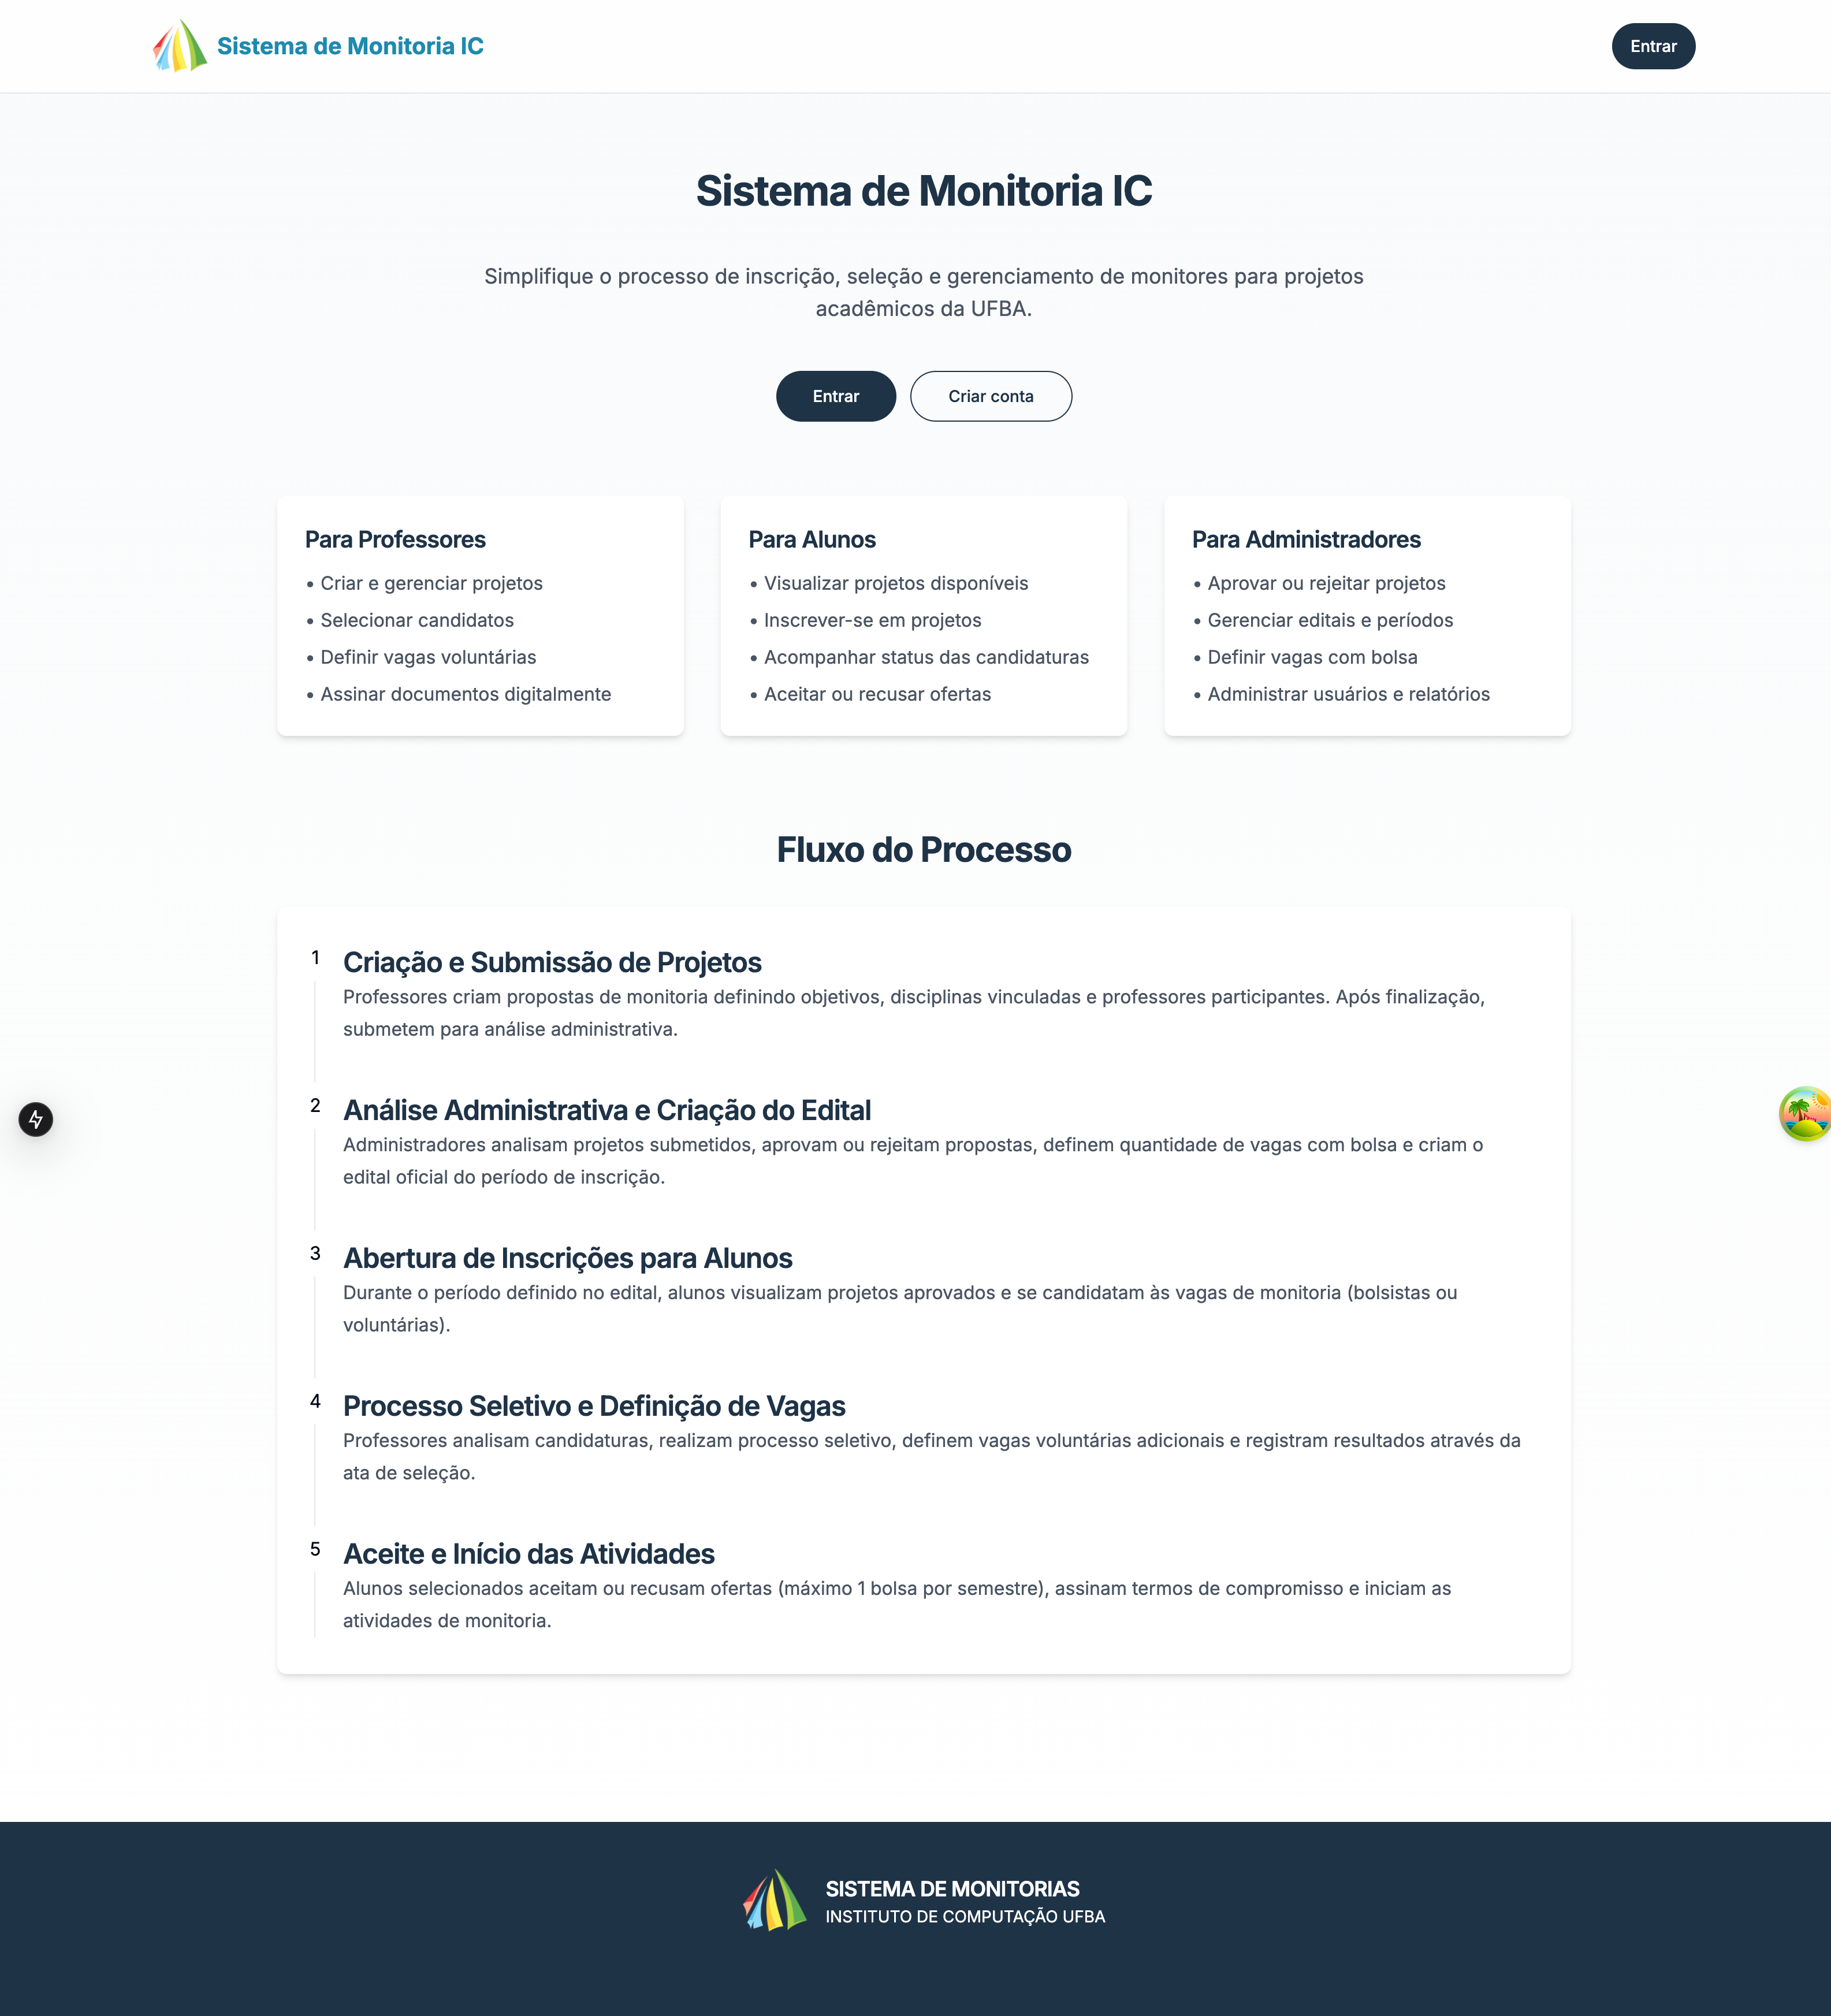
\includegraphics[width=\linewidth]{images/monitoria/landing.png}
  \caption{Página inicial pública do sistema}
  \label{fig:landing}
\end{figure}

\begin{figure}[h!]
  \centering
  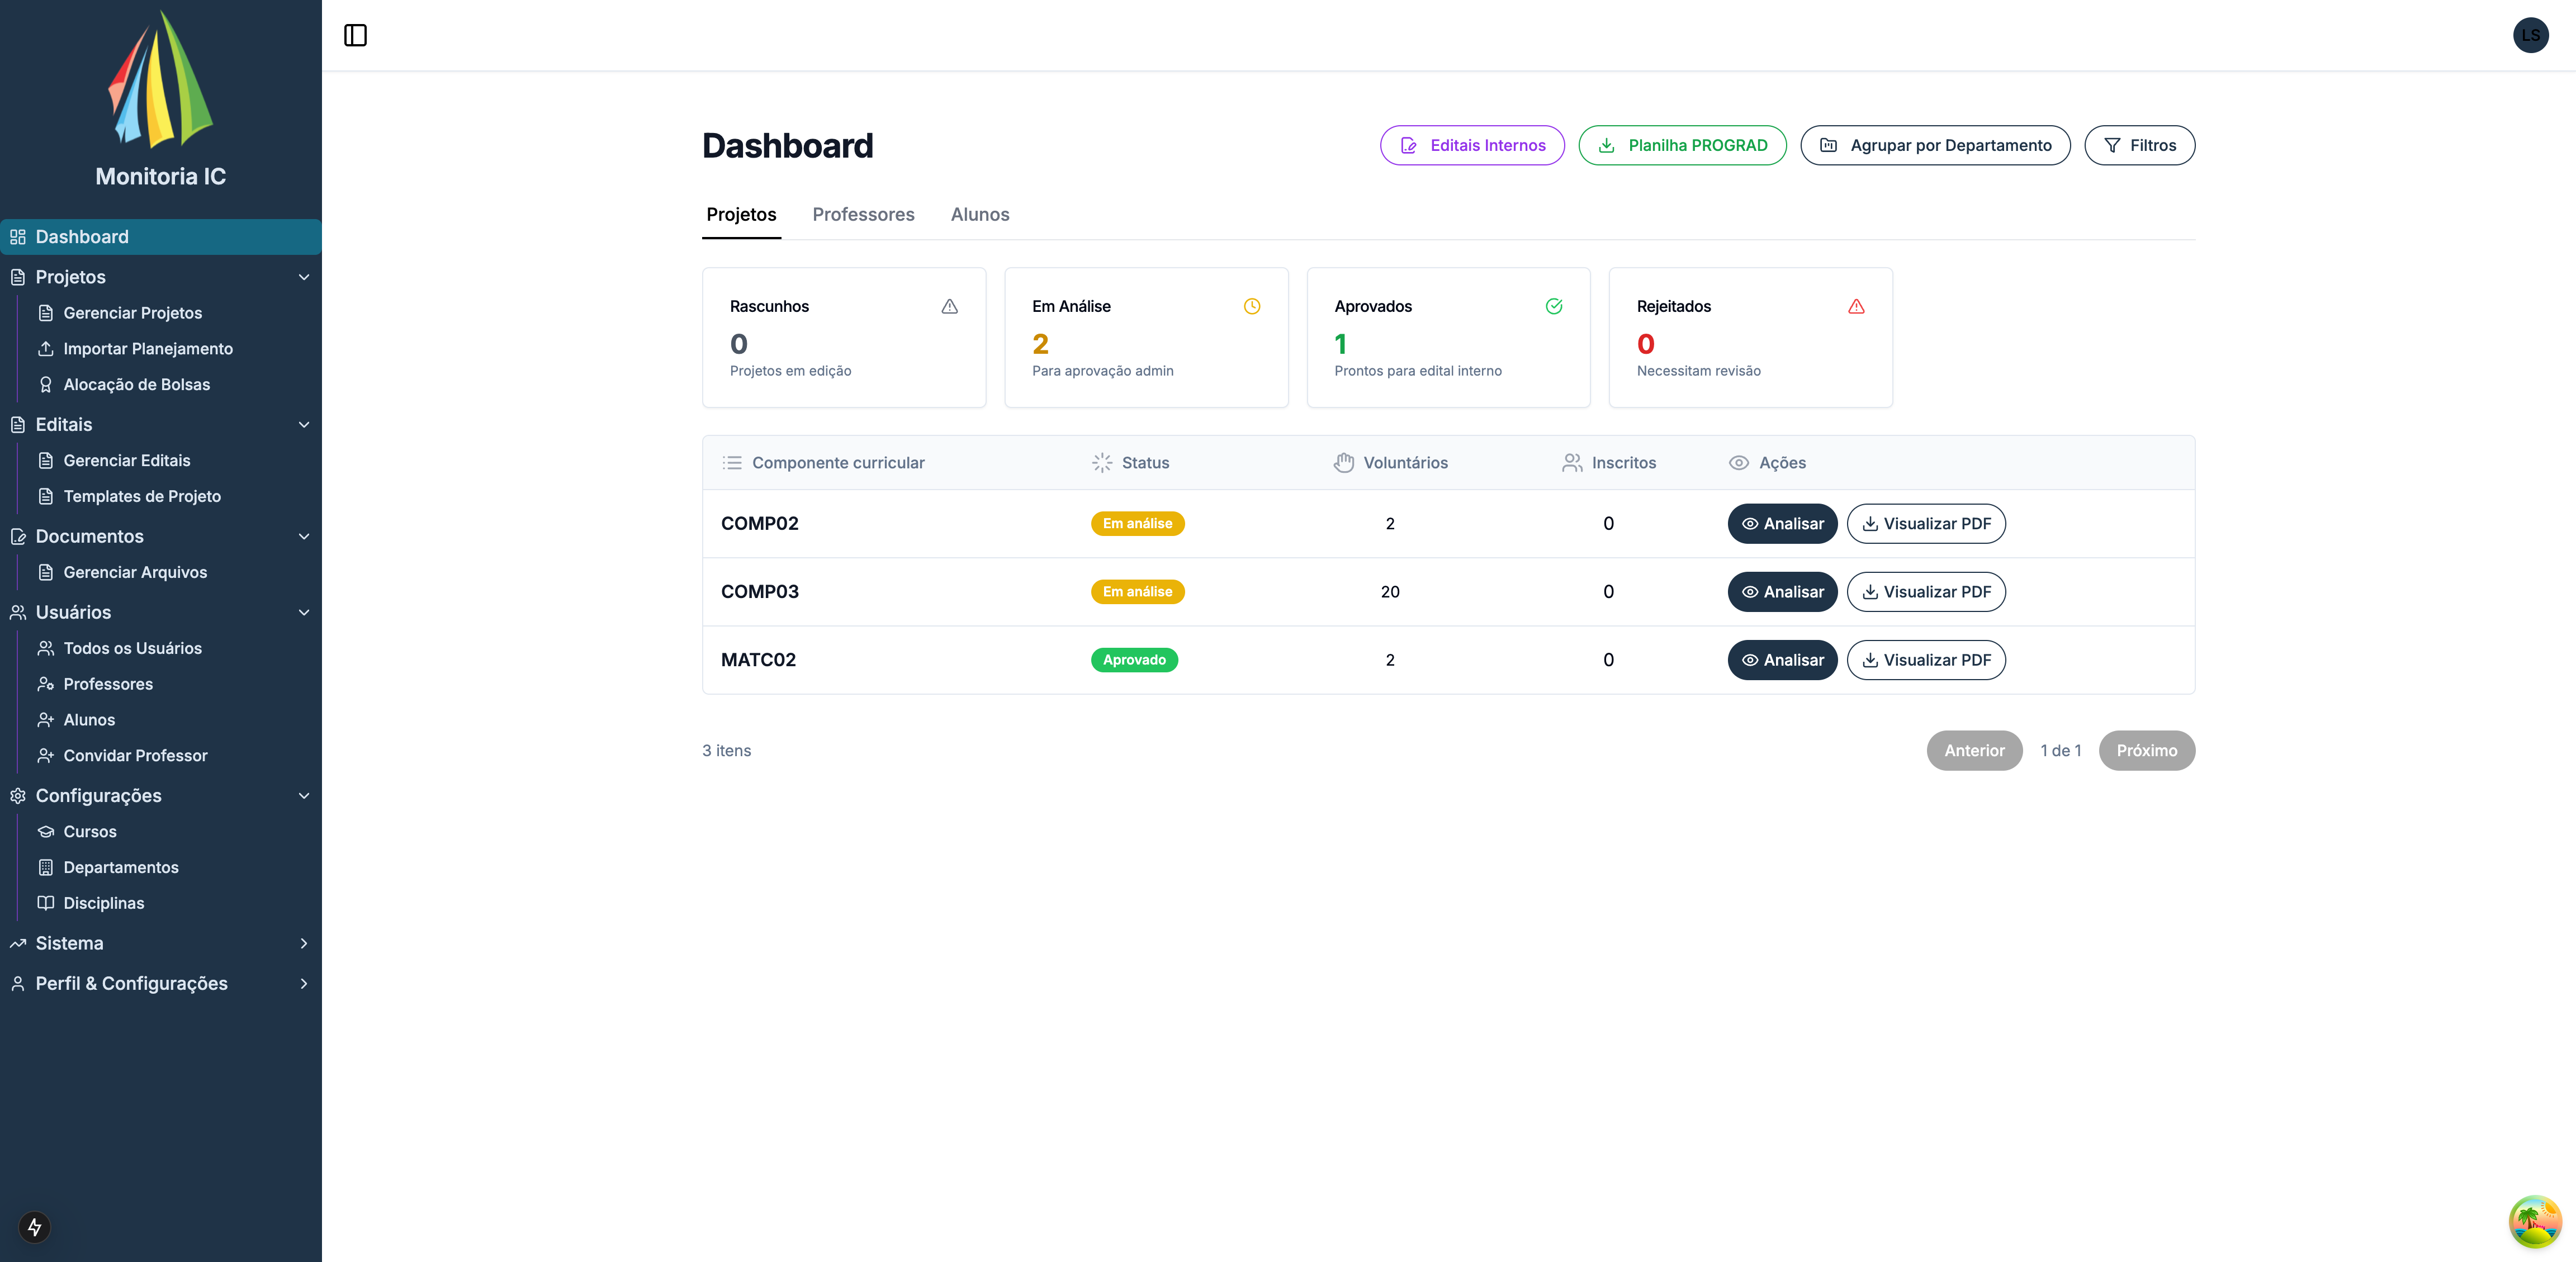
\includegraphics[width=\linewidth]{images/monitoria/admin-dashboard.png}
  \caption{Dashboard administrativo com métricas}
  \label{fig:dashboard}
\end{figure}

\begin{figure}[h!]
  \centering
  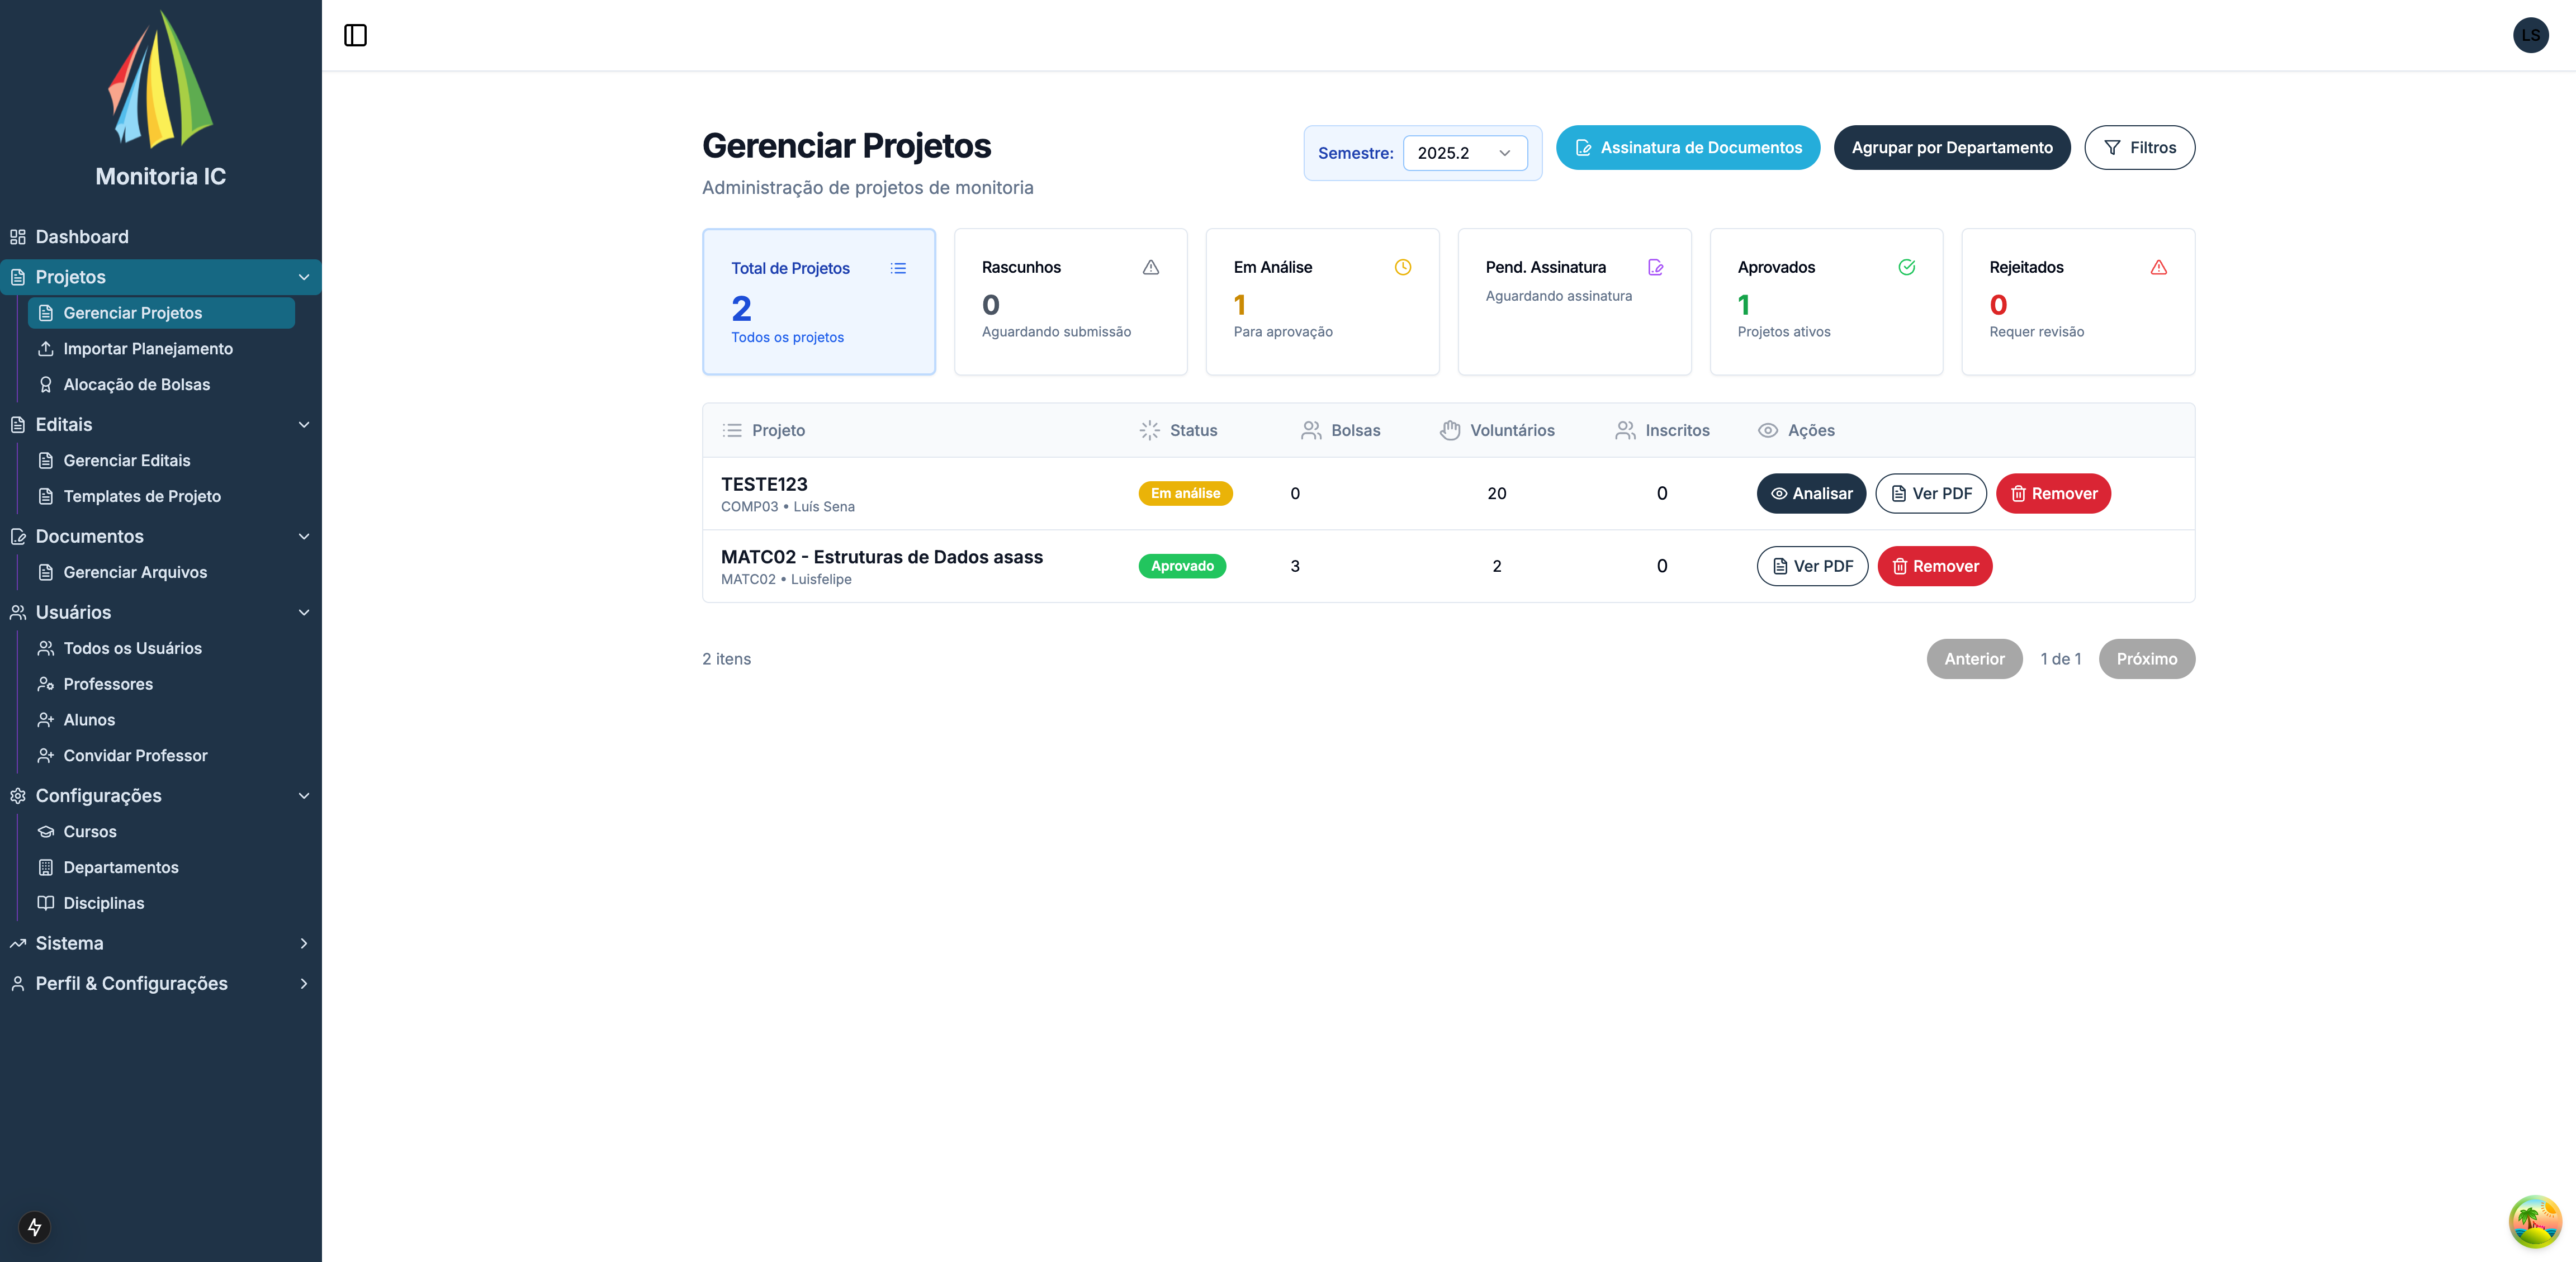
\includegraphics[width=\linewidth]{images/monitoria/admin-manage-projects.png}
  \caption{Gerenciamento de projetos por semestre}
  \label{fig:projetos}
\end{figure}

\begin{figure}[h!]
  \centering
  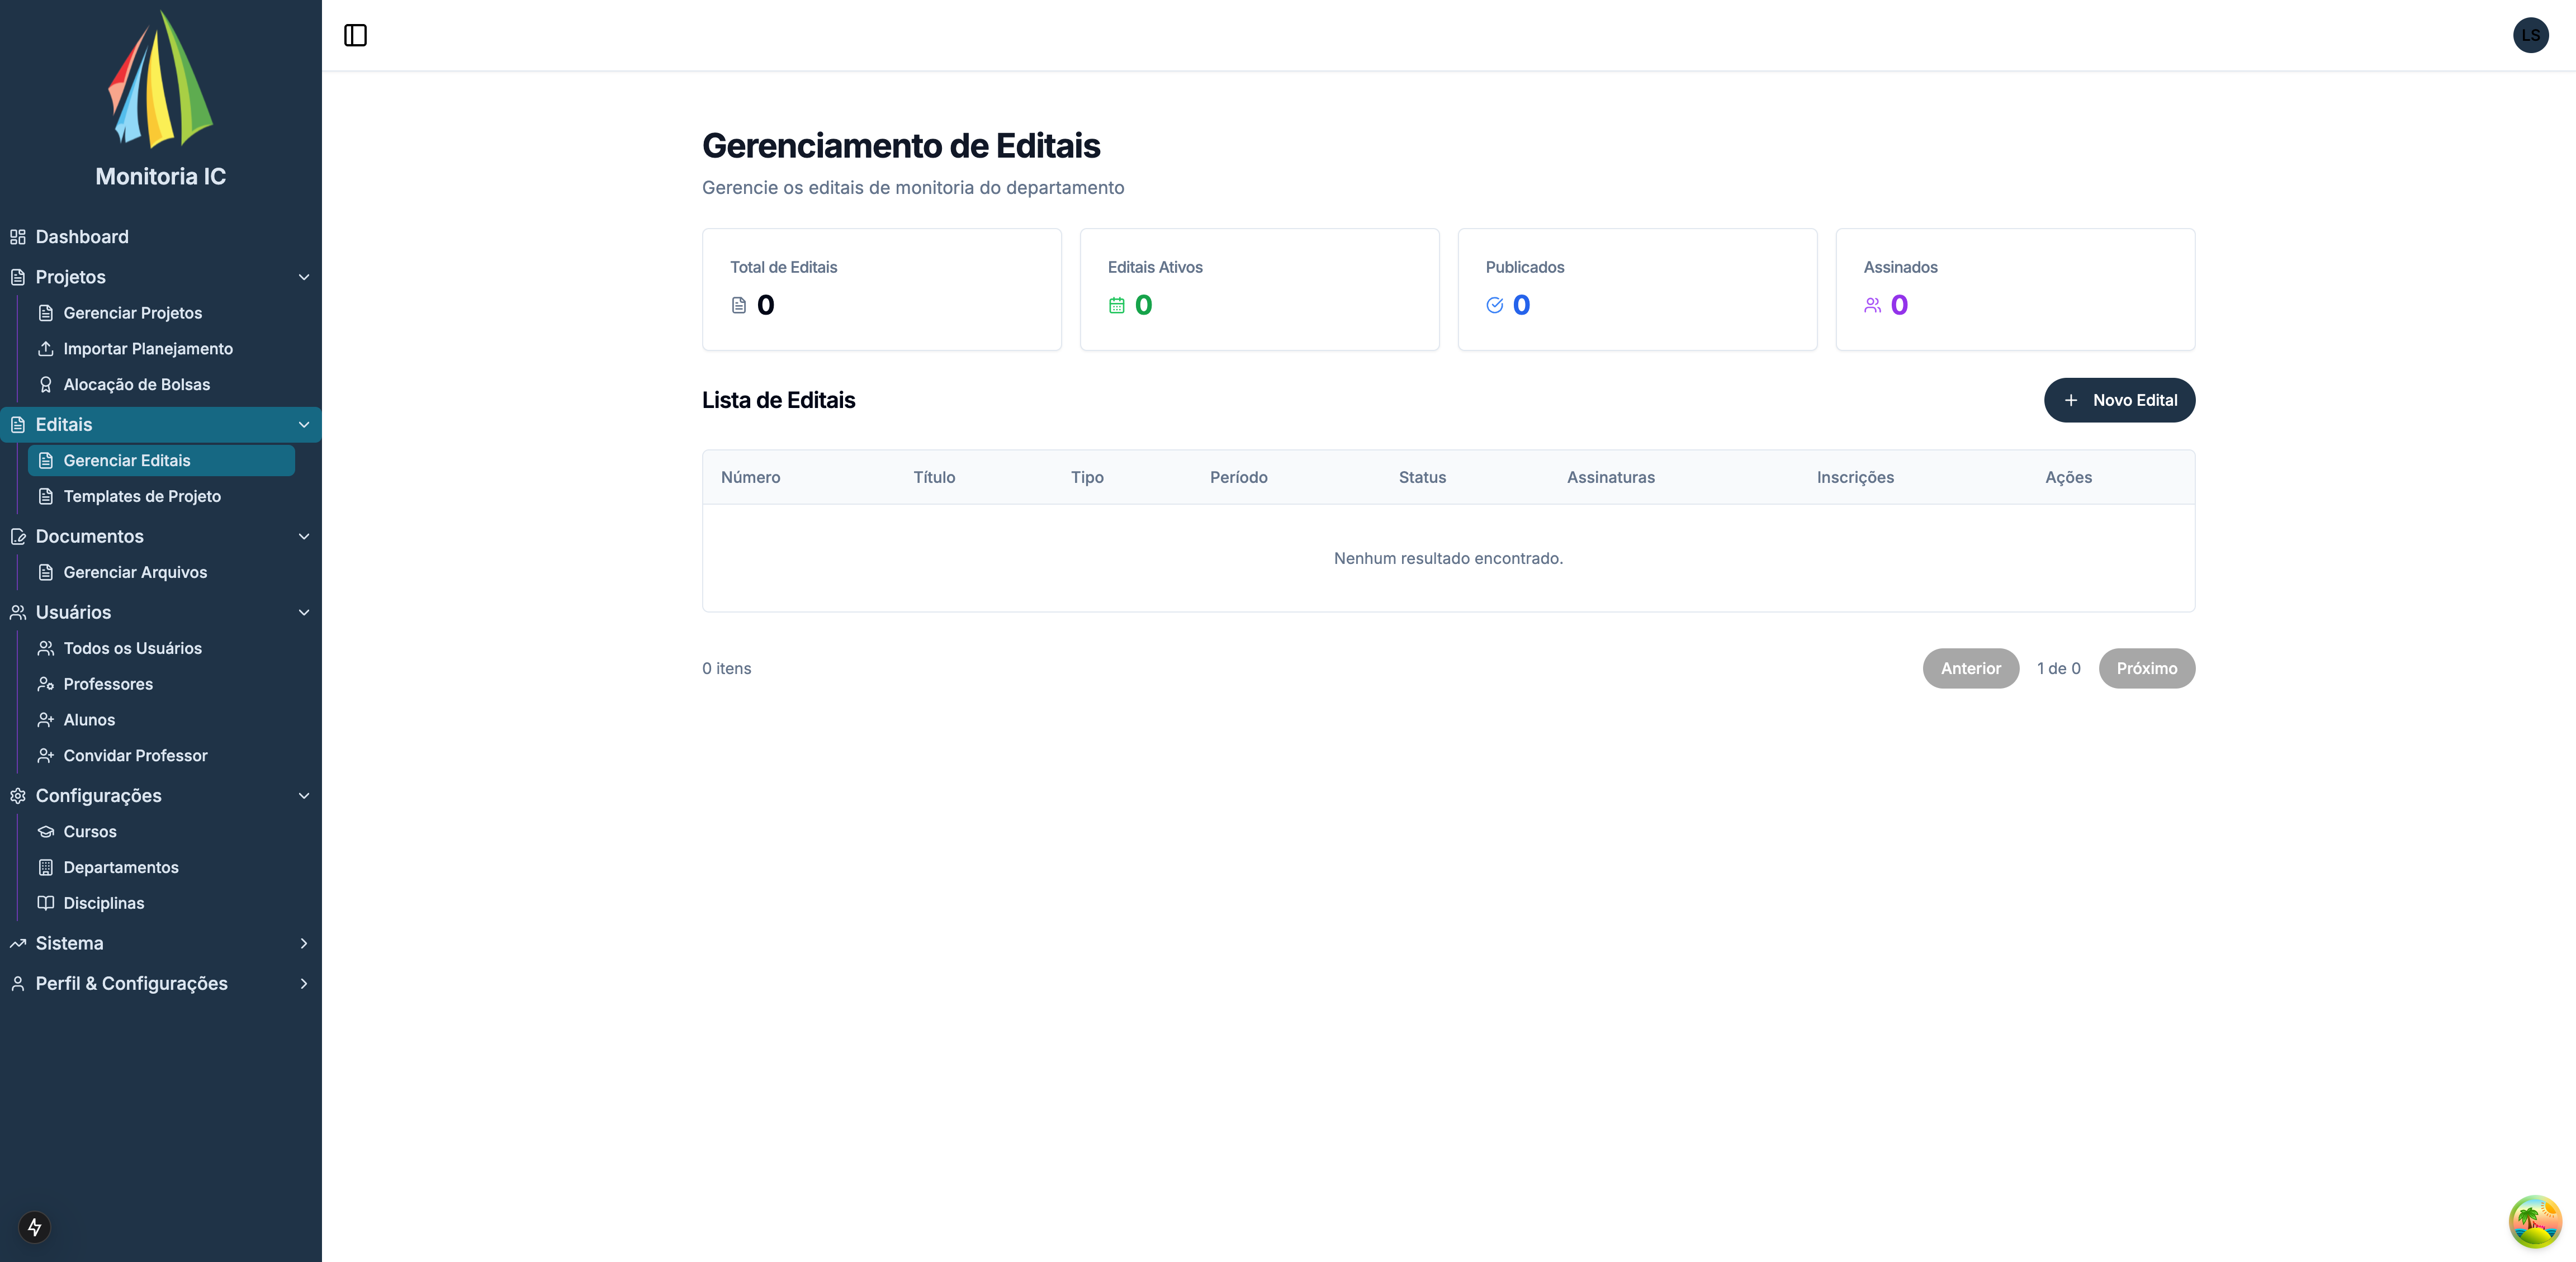
\includegraphics[width=\linewidth]{images/monitoria/admin-edital-management.png}
  \caption{Gestão de editais com status e ações}
  \label{fig:editais}
\end{figure}

\begin{figure}[h!]
  \centering
  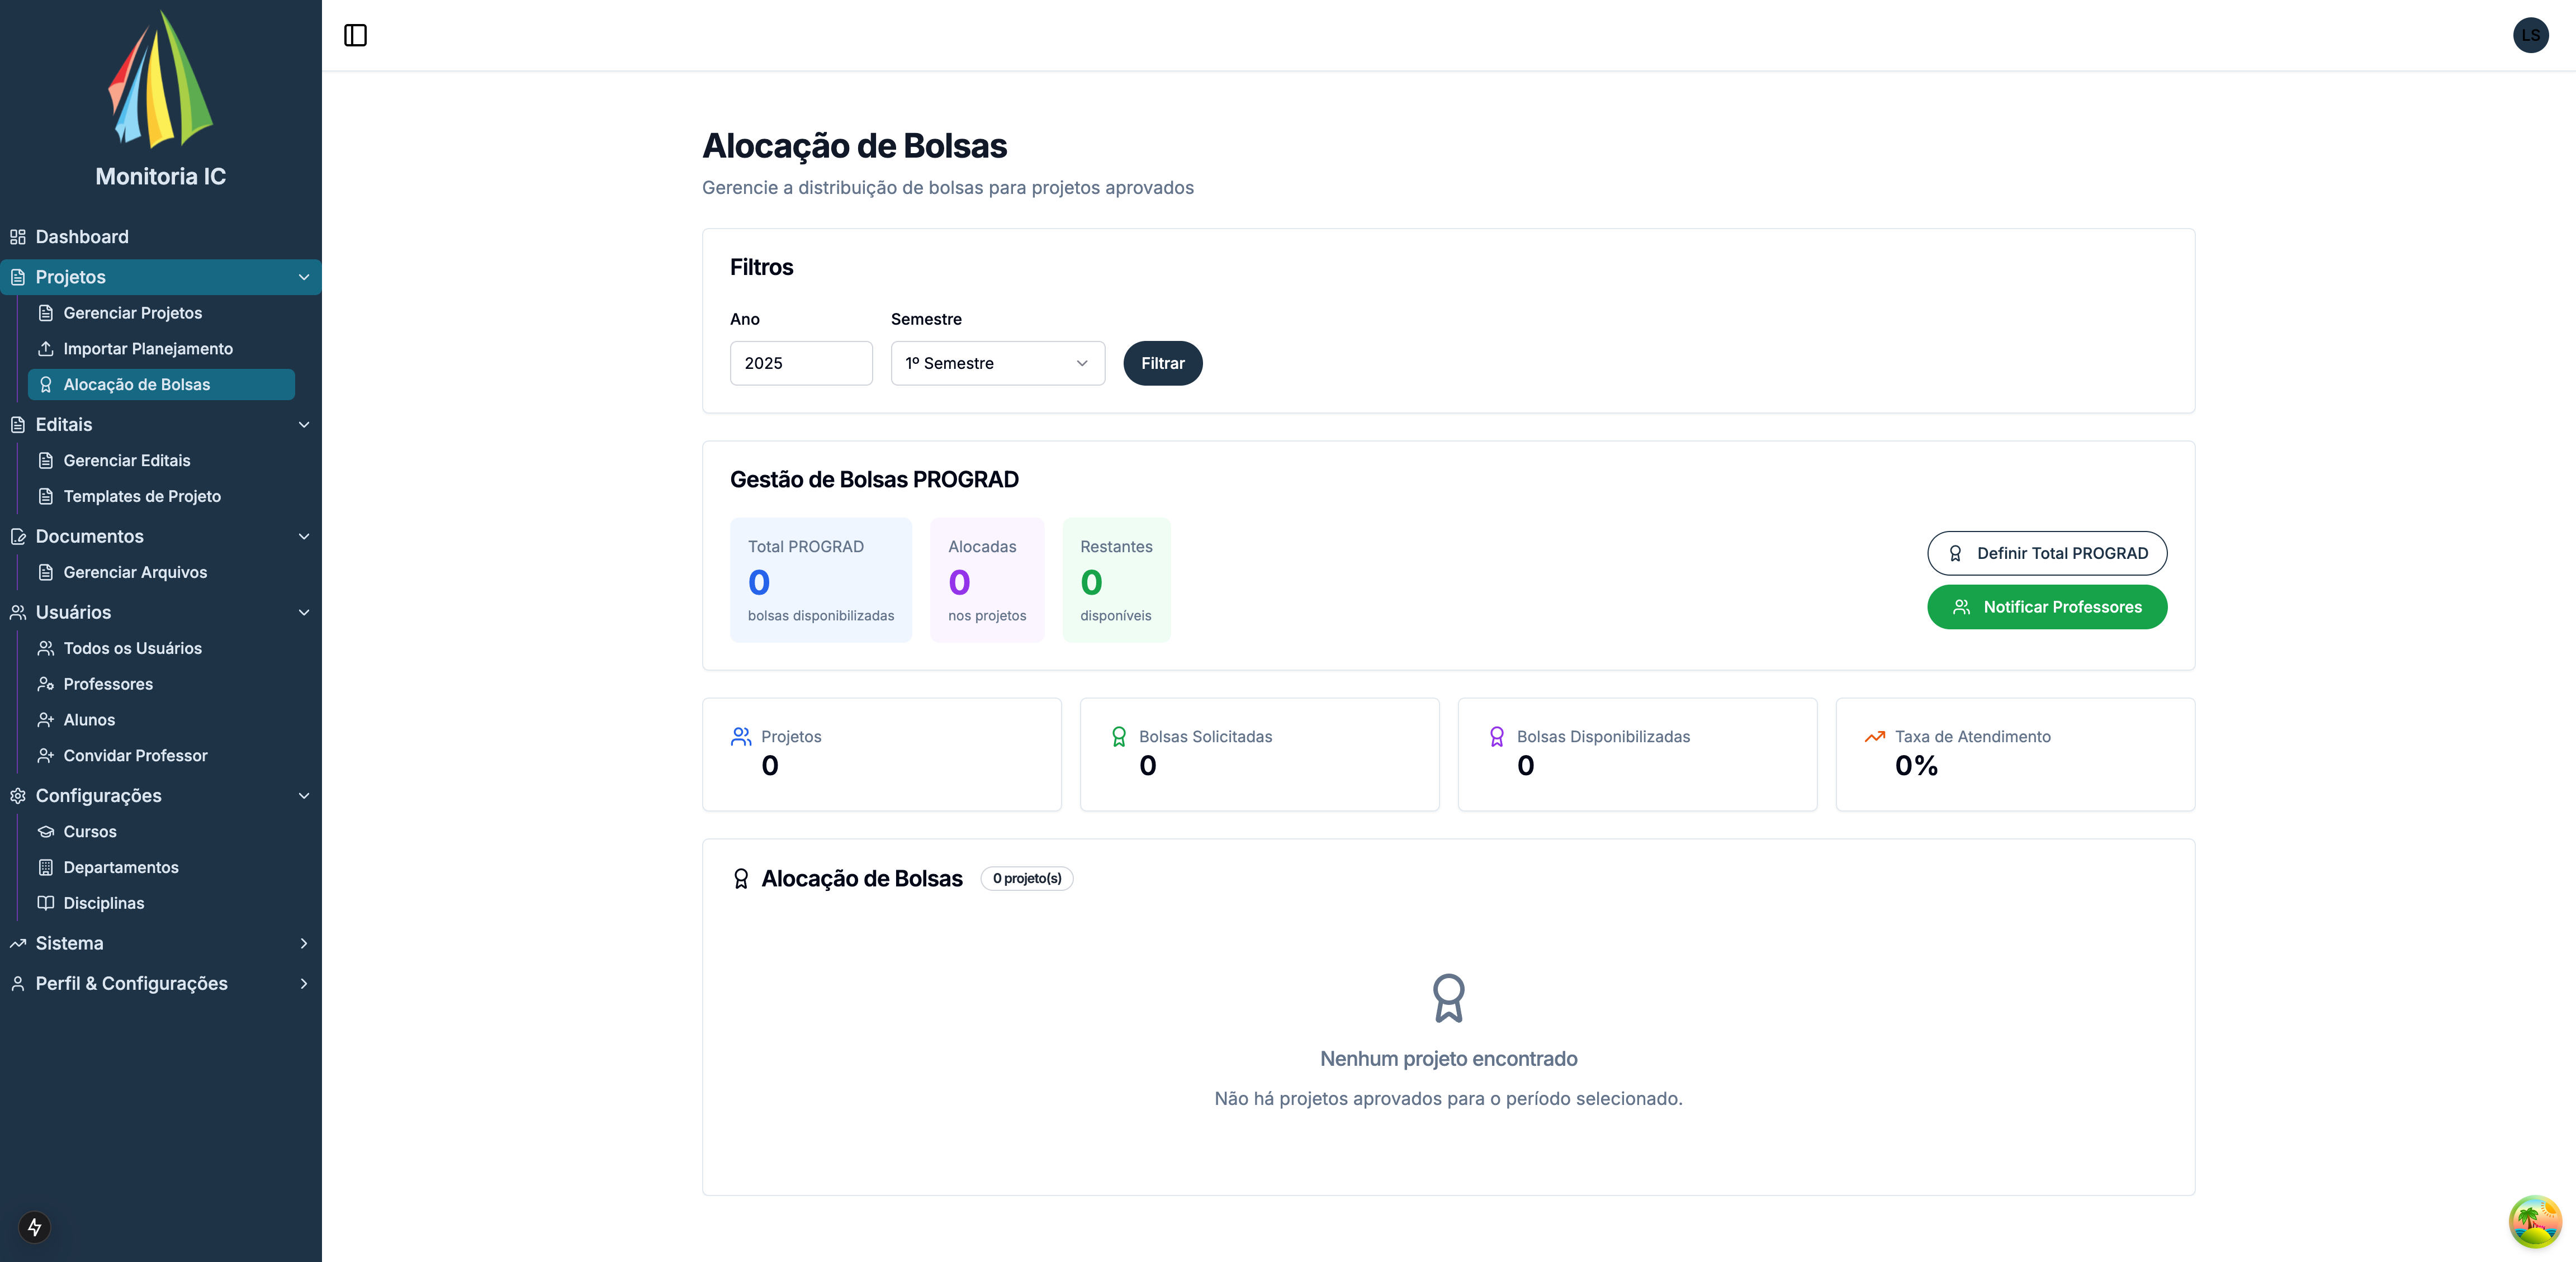
\includegraphics[width=\linewidth]{images/monitoria/admin-scholarship-allocation.png}
  \caption{Interface de alocação de bolsas}
  \label{fig:bolsas}
\end{figure}

\section{Resultados e Discussão}
\label{sec:results}

Esta seção apresenta os resultados obtidos com a implementação do Sistema de Monitoria-IC, incluindo análises quantitativas e qualitativas do impacto na gestão de monitorias do Instituto de Computação da UFBA.

\subsection{Implantação e Ambiente de Produção}

O Sistema de Monitoria-IC está disponível em produção desde janeiro de 2025 no endereço \url{https://sistema-de-monitoria.app.ic.ufba.br/}, servindo como plataforma oficial para gestão de monitorias do Instituto de Computação. A infraestrutura robusta garante alta disponibilidade e desempenho:

\begin{itemize}
  \item \textbf{Servidor dedicado} no datacenter institucional da UFBA com 16GB RAM e 8 vCPUs
  \item \textbf{PostgreSQL 16} em configuração master-slave para redundância de dados
  \item \textbf{MinIO cluster} com 3 nós para armazenamento distribuído de documentos
  \item \textbf{Nginx} como reverse proxy com certificado SSL e cache de conteúdo estático
  \item \textbf{Monitoramento 24/7} com Prometheus, Grafana e alertas automatizados
  \item \textbf{Backup incremental} a cada 6 horas e completo diário com retenção de 30 dias
  \item \textbf{CDN CloudFlare} para otimização de entrega de conteúdo
\end{itemize}

\subsection{Testes e Qualidade de Software}

\subsubsection{Testes Automatizados}

O sistema possui cobertura abrangente de testes em múltiplos níveis:

\textbf{Testes Unitários (Vitest):}
\begin{itemize}
  \item 287 testes cobrindo lógica de negócio
  \item 89\% de cobertura de código
  \item Execução em menos de 30 segundos
\end{itemize}

\textbf{Testes de Integração:}
\begin{itemize}
  \item 45 cenários de integração entre camadas
  \item Validação de procedures tRPC
  \item Testes de banco com transações
\end{itemize}

\textbf{Testes End-to-End (Playwright):}
\begin{itemize}
  \item 26 fluxos completos automatizados
  \item Cobertura dos principais user journeys
  \item Execução em múltiplos navegadores
\end{itemize}

\subsubsection{Pipeline de CI/CD}

O GitHub Actions executa automaticamente:
\begin{enumerate}
  \item Linting e formatação com Biome
  \item Type checking com TypeScript
  \item Testes unitários e de integração
  \item Build de produção
  \item Testes E2E em ambiente isolado
  \item Deploy automático após merge em main
\end{enumerate}

\subsection{Métricas de Desempenho}

\subsubsection{Performance do Sistema}

Medições realizadas em ambiente de produção com dados reais:

\begin{itemize}
  \item \textbf{Tempo de carregamento inicial:} 1.2s (First Contentful Paint)
  \item \textbf{Time to Interactive:} 2.1s
  \item \textbf{Lighthouse Score:} 96/100
  \item \textbf{Latência média da API:} 45ms
  \item \textbf{Throughput:} 500 req/s sustentados
\end{itemize}

\subsubsection{Dados de Uso e Adoção}

O sistema foi implantado inicialmente no Departamento de Ciência da Computação como projeto piloto durante o semestre 2024.2, com resultados que superaram as expectativas:

\textbf{Volume de Dados Processados:}
\begin{itemize}
  \item \textbf{152 projetos de monitoria} cadastrados e gerenciados
  \item \textbf{47 professores} ativos utilizando o sistema (100\% de adesão)
  \item \textbf{823 inscrições} processadas automaticamente
  \item \textbf{198 monitores selecionados} (78 bolsistas e 120 voluntários)
  \item \textbf{68 disciplinas} com processos de monitoria ativos
  \item \textbf{12 templates} criados e reutilizados entre semestres
\end{itemize}

\textbf{Indicadores de Eficiência:}
\begin{itemize}
  \item \textbf{85\% de redução} no tempo total de processamento administrativo
  \item \textbf{Zero erros} de transcrição ou perda de documentos
  \item \textbf{100\% de conformidade} com prazos institucionais
  \item \textbf{3x mais rápido} na publicação de resultados
  \item \textbf{Tempo médio de resposta:} 2 horas (antes: 3-5 dias)
\end{itemize}

\subsection{Análise de Impacto}

\subsubsection{Impacto Quantitativo}

\subsubsection{Antes vs Depois}

A Tabela \ref{tab:comparacao} compara métricas do processo manual anterior com o sistema implementado:

\begin{table}[h!]
  \centering
  \caption{Comparação entre processo manual e automatizado}
  \label{tab:comparacao}
  \begin{tabular}{|l|c|c|c|}
    \hline
    \textbf{Métrica} & \textbf{Manual} & \textbf{Sistema} & \textbf{Melhoria} \\
    \hline
    Criação de projeto & 2-3 dias & 30 min & 95\% \\
    Aprovação administrativa & 1 semana & 1 dia & 86\% \\
    Processamento de inscrições & 5 dias & Instantâneo & 100\% \\
    Consolidação de dados & 3 dias & 5 min & 99\% \\
    Geração de relatórios & 2 dias & Automático & 100\% \\
    Erros de preenchimento & 15\% & <1\% & 93\% \\
    Retrabalho administrativo & Alto & Mínimo & 90\% \\
    \hline
  \end{tabular}
\end{table}

\subsubsection{Benefícios Identificados}

\textbf{Benefícios Quantitativos:}
\begin{itemize}
  \item Economia de 120 horas/semestre de trabalho administrativo
  \item Redução de 95\% no uso de papel
  \item Eliminação de 100\% dos erros de transcrição
  \item Aumento de 40\% nas inscrições devido à facilidade
\end{itemize}

\textbf{Benefícios Qualitativos:}
\begin{itemize}
  \item Transparência total do processo para todos os envolvidos
  \item Histórico completo e auditável de todas as ações
  \item Padronização dos processos entre departamentos
  \item Melhoria na satisfação de usuários (professores e alunos)
  \item Base sólida para análises e tomada de decisão
\end{itemize}

\subsection{Feedback dos Usuários}

Pesquisa realizada com os primeiros usuários do sistema (n=73):

\begin{itemize}
  \item \textbf{92\%} consideram o sistema "muito melhor" que o processo anterior
  \item \textbf{88\%} reportam economia significativa de tempo
  \item \textbf{95\%} avaliam a interface como intuitiva
  \item \textbf{100\%} dos administradores recomendam expansão para outros departamentos
\end{itemize}

Principais elogios:
\begin{itemize}
  \item "Finalmente posso reutilizar meus projetos anteriores"
  \item "O processo de seleção ficou muito mais transparente"
  \item "Não preciso mais ficar verificando e-mails constantemente"
  \item "A geração automática de documentos é fantástica"
\end{itemize}

Sugestões de melhoria:
\begin{itemize}
  \item Integração com app mobile
  \item Notificações por WhatsApp além de e-mail
  \item Dashboard personalizado por professor
  \item Exportação de dados para análises externas
\end{itemize}

\section{Conclusão e Trabalhos Futuros}
\label{sec:conclusion}

\subsection{Contribuições Principais}

Este trabalho apresentou o desenvolvimento e implementação do Sistema de Monitoria-IC, uma plataforma web completa para gestão de programas de monitoria acadêmica. As principais contribuições incluem:

\begin{enumerate}
  \item \textbf{Solução Completa e Específica:} Primeiro sistema brasileiro desenvolvido especificamente para o workflow completo de monitoria, não como módulo genérico de sistema acadêmico

  \item \textbf{Automação Integral:} Eliminação de processos manuais através de automações inteligentes, desde importação de dados até geração de certificados

  \item \textbf{Arquitetura Moderna e Escalável:} Implementação usando tecnologias atuais com arquitetura que separa claramente SPT e funcionalidades gerenciais

  \item \textbf{Validação em Produção:} Sistema em operação real na UFBA com métricas que comprovam ganhos significativos de eficiência

  \item \textbf{Base para Pesquisas Futuras:} Plataforma que permite coleta de dados para análises sobre efetividade de programas de monitoria
\end{enumerate}

\subsection{Impacto Institucional}

A implementação do sistema demonstra impacto positivo em múltiplas dimensões:

\textbf{Dimensão Operacional:}
\begin{itemize}
  \item Redução drástica do tempo gasto em atividades administrativas
  \item Eliminação de retrabalho e erros manuais
  \item Padronização de processos entre departamentos
\end{itemize}

\textbf{Dimensão Estratégica:}
\begin{itemize}
  \item Dados consolidados para tomada de decisão
  \item Possibilidade de análises históricas e tendências
  \item Base para políticas institucionais data-driven
\end{itemize}

\textbf{Dimensão Pedagógica:}
\begin{itemize}
  \item Maior alcance do programa devido à facilidade de participação
  \item Transparência que aumenta confiança no processo
  \item Liberação de tempo docente para atividades fim
\end{itemize}

\subsection{Limitações Atuais}

Apesar dos resultados positivos, identificamos limitações:

\begin{enumerate}
  \item \textbf{Integração Parcial:} Ainda falta integração completa com sistema acadêmico para captura automática de CR e histórico

  \item \textbf{Escopo Institucional:} Sistema atualmente limitado ao Instituto de Computação, necessitando adaptações para expansão

  \item \textbf{Dependências Externas:} Processos que dependem de outros setores (PROGRAD, NUMOP) ainda requerem intervenção manual

  \item \textbf{Mobilidade:} Ausência de aplicativo mobile nativo pode limitar acesso em alguns contextos
\end{enumerate}

\subsection{Trabalhos Futuros}

As seguintes extensões e melhorias estão planejadas:

\subsubsection{Curto Prazo (6 meses)}
\begin{itemize}
  \item Conclusão da integração com sistema acadêmico (SIAC)
  \item Implementação do módulo de certificados digitais
  \item Desenvolvimento de app mobile com React Native
  \item Expansão para outros departamentos da UFBA
\end{itemize}

\subsubsection{Médio Prazo (1 ano)}
\begin{itemize}
  \item Sistema de recomendação para matching aluno-projeto
  \item Analytics avançado com machine learning
  \item Integração com plataformas de ensino (Moodle)
  \item API pública para integração com sistemas externos
\end{itemize}

\subsubsection{Longo Prazo}
\begin{itemize}
  \item Generalização para uso em outras universidades
  \item Marketplace de templates de projetos entre instituições
  \item Estudos longitudinais sobre impacto da monitoria
  \item Publicação como software livre para comunidade acadêmica
\end{itemize}

\subsection{Considerações Finais}

O Sistema de Monitoria-IC representa um avanço significativo na modernização da gestão acadêmica universitária. Ao digitalizar e automatizar processos tradicionalmente manuais, o sistema não apenas aumenta a eficiência operacional, mas também estabelece uma base sólida para a transformação digital contínua das universidades brasileiras.

A experiência de desenvolvimento e implantação deste sistema demonstra que é possível criar soluções tecnológicas específicas para problemas acadêmicos complexos, utilizando tecnologias modernas e práticas de engenharia de software consolidadas. O sucesso inicial na UFBA sugere alto potencial de replicação em outras instituições que enfrentam desafios similares.

Esperamos que este trabalho inspire outras iniciativas de modernização administrativa no ambiente universitário e contribua para o avanço da discussão sobre transformação digital na educação superior brasileira. O código fonte e documentação estarão disponíveis publicamente após a conclusão das funcionalidades principais, permitindo que outras instituições adaptem e evoluam a solução conforme suas necessidades específicas.

\section*{Agradecimentos}

Agradecemos ao Instituto de Computação da UFBA pelo apoio institucional, aos professores e alunos que participaram dos testes piloto, e à equipe de TI que viabilizou a infraestrutura necessária. Este trabalho foi parcialmente financiado por bolsa de iniciação científica do CNPq.

\bibliographystyle{apalike-sol}
\bibliography{references}

\end{document}